\chapter{Separation of Variables for the Hydrogen Molecular Ion}

In this chapter, we review analytic methods\cite{Bates1,Bates2,Slater} used to obtain 
solutions of the time-independent Schrodinger equation for 
the hydrogen molecular.

As we will apply a similar method to treat the hydrogen molecular ions in 2D,
we first review the methodology of Bates used to calculate the lowest electronic eigenstates and eigenvalues for the $ {\rm H}_2^{+} $ system in 3D. \footnote {In this section we
use atomic (Hatree) units, unless otherwise stated.}

The hydrogen molecular ion, and similar systems ( such as $ {\rm HeH}^{+} $) are one of the few that allow a full analytic quantum mechanical description. Although its
solutions do not exist in the closed form, they can be expressed as a convergent infinite series.  Wasserman in his thesis \cite{ExperimentalBates2} in 1963 reports that while the existence of $ {\rm H}_2^{+} $ has been verified, no  discrete spectrum of the  $ {\rm H}_2^{+} $ has been observed  In the same thesis, Wasserman reports that the ionization potential of $ {\rm H}_2^{+} $ has been measured and shows good agreement with the theoretical calculations. However, in 1989 Carrington, McNab and Montgomerie report \cite{ExperimentalBates3} that the radio frequency hyperfine transitions of the $ {\rm H}_2^{+} $ have been measured. They note that the $ {\rm H}_2^{+} $  is highly reactive and therefore hard to keep in the lab.

As a three-body problem, containing two protons and an electron,
the Schrodinger PDE can be separated by expressing it in an elliptical coordinate system. Unfortunately, there does not exist a closed form representation for the eigenvalues and one must resort to numerical methods in their calculation.
Bates et al. \cite{Bates1}\cite{Bates2} did not provide numerical codes used the evaluation of eigenvalues. Instead, they used an expanded fraction method for calculating the latter with the desired level of precision. The paper\cite{Bates2} does not report on the details of those calculations, and so in this thesis we provide an alternative description. We will compare
 the results obtained here with those reported in\cite{Bates2}. Harmony with with those reported in\cite{Bates2} will provide 
 confidence in the fidelity of the analogous calculations in 2D.

We use Hartree Atomic Units \eqref{Atomic}, in all equations. In this system the numerical values of the following fundamental constants are 1:
\setlength{\mathindent}{0pt}
\begin{equation}\label{Atomic}
\begin{split}
    & \text{Electron mass:}\ &\ m_e = 1 \\ 
    & \text{Electron charge:}\ &\ e = 1 \\
    & \text{Reduced Planck constant:}\ &\ \hbar = 1 \\
    & \text{Coulomb's constant:}\ &\ \frac{1}{4\pi\epsilon_0} = 1
\end{split}
\end{equation}

In addition, in equations, variables that represent vectors are typeset in \textbf{bold}. A caret ($ \hat{}\ $ ) above a symbol indicates that the symbol is an operator.

The only place where we specifically will not be using Atomic units will be in the following derivation, where we do transformation of the molecular Hamiltonian into a Jacobian coordinate system. Since some terms will contain reduced mass, we want to keep the units intact.

\section{Description}
The starting point is the Schrodinger equation for the hydrogen molecular ion in 3D. We 
seek stationary states for non-relativistic motion, and neglect the spin degrees of freedom. With these assumptions the Schrodinger equation for such a system is given by:
\begin{equation}\label{sch1}
\hat{H}^{'}\psi\left(\mathbf{R},\mathbf{x}\right) = E\,\psi\left(\mathbf{R},\mathbf{x}\right).
\end{equation}
$ \hat{H} $ represents total Hamiltonian and $ \psi\left(\mathbf{R},\mathbf{x}\right) $ is an eigenstate wavefunction. It is a function of both the collective nuclear coordinates $ \mathbf{R} $,  and electronic coordinates $\mathbf{x} $. Of course, since we are considering the hydrogen molecular ion, $\mathbf{x} $ is the coordinate of a single electron.

The hydrogen molecular ion $ {\rm H}_2^{+} $ is composed of 2 protons and a single electron. Thus, as we are neglecting relativistic effects and spin, its Hamiltonian is given as:
\begin{equation}\label{hh}
\hat{H} = \hat{T}_n + \hat{T}_e + \hat{V}_{en} + \hat{V}_{nn}. 
\end{equation}

The terms in the Hamiltonian are as follows:

The kinetic energy of the protons:
\begin{equation}`
\begin{split}
 \hat{T}_n = - \frac{\hbar^2}{2M}\sum_{i=1}^2{\nabla_{R_i}^2 } = -\frac{1}{2M}\sum_{i=1}^2{\hat{P}_i^2 }
\end{split}
\end{equation}

The kinetic energy of the electron:
\begin{equation}
\begin{split}
 \hat{T}_e= -\frac{\hbar^2}{2m}\nabla_{x}^2 = \frac{1}{2m}\hat{p}^2  \\[.8em]
\end{split}
\end{equation}

The potential energy between the electron and the nuclei, i.e. the total Coulomb electron - nuclei attraction:
\begin{equation}
\begin{split}
 \hat{V}_{en} = -\sum_{i=1}^2{\left|\mathbf{R}_i - \mathbf{x}\right| }   
\end{split}
\end{equation}

Potential energy (operators) between the nuclei - the total Coulomb proton - proton repulsion. 
\begin{equation}
\begin{split}
 \hat{V}_{nn} =  \frac{e^2}{\left|\mathbf{R}_1 - \mathbf{R}_2\right| } 
\end{split}
\end{equation}
The second term in the equation above represents the operator expression.

In the equations above, $ \mathbf{R}_i,\,\, i = 1,2 $ and $ M $ represents the coordinates and mass of the nuclei (protons) $1,2$ respectively, and $ \mathbf{x} $ and $ m $ are the coordinates and mass of the electron, respectively. Coordinates are defined with respect to a common origin in a space fixed frame.

It is convenient to separate the motion of the center of mass from the motion of the point particles. A similar approach can be applied for the quantum case. We show in Appendix A that the motion of the center of mass will be a plane wave, which possess a well defined momentum and which is not square integrable. That makes the position of the center of mass equally probable in the hole space, which agrees with the Heisenberg uncertainty principle.

In the appendix A we define $ \chi(\mathbf{R}) $ as the wavefunction representing the motion of the nuclei. We then  obtain:
\begin{equation}
\chi(\mathbf{R}) = \frac{1}{(2\pi\hbar)^{3/2}}e^{\frac{i}{\hbar}\sqrt{2ME_{CM}}\mathbf{R}}
\end{equation}

Therefore, we proceed to transform the Hamiltonian into a Jacobian coordinate system, following \cite{ZygelmanDalgarno1}. The outcome of this procedure will be the transformation of the wave function as $\psi(\mathbf{R}_i, \mathbf{r}) \rightarrow \psi(\mathbf{R}_{CM}, \mathbf{R}, \mathbf{r}) $ where the $ \mathbf{R}_{CM} $ is the coordinate of the center of the mass, $ R $ is the distance between nuclei and $ \mathbf{r} $ is an electron coordinate.
We choose the coordinates as:

\begin{equation}
\begin{split}
& \mathbf{R}_{CM} = \frac{M\,\mathbf{R}_1 + M\,\mathbf{R}_2 + m\,\mathbf{x}}{2M + m} \\[.8em]
& \mathbf{R} = \mathbf{R}_1 - \mathbf{R}_2 \\[.8em]
& \mathbf{r} = \mathbf{x} - \frac{\mathbf{R}_1 + \mathbf{R}_2}{2}
\end{split}
\end{equation}

\begin{figure}
  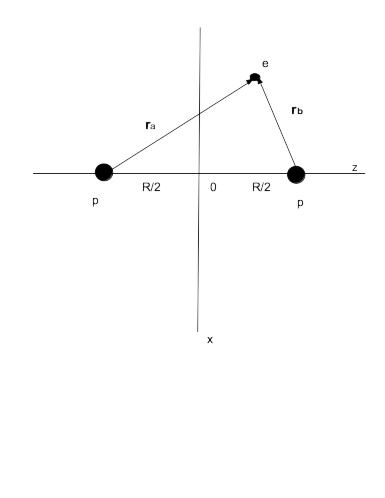
\includegraphics{H2Ion3D.png}
  \caption{$ H_2 $ Ion}\label{h2ion3d}
\end{figure}

Now following \cite{ZygelmanDalgarno1},\cite{Greg}, we obtain the expression of the molecular Hamiltonian in the new coordinates,
\begin{equation}
\begin{split}
& H^{'} = T_{CM} + T_{KE} + H_{AD} \,\,\,\,\text{ where } \\[.8em]
& \text{Motion of the center of the mass which can be separated from the total energy of the nuclei: } \\[.8em]
& T_{CM} = -\frac{1}{2(2M +m)}\nabla_{CM}^{2} \\[.8em]
& \text{ The relative motion of the nuclei } \\[.8em]
& T_{KE} = -\frac{1}{2\mu}\nabla_R^2 \\[.8em]
& \text{where} \\[.8em]
& \mu = \frac{M}{2}\,\,\text{ is a reduced mass of the 'bare' nuclei}
\end{split}
\end{equation}
and
\begin{equation}\label{HAD}
\begin{split}
    & \text{ The adiabatic Hamiltonian: } \\[.8em]
& H_{AD} = -\frac{1}{2m}\nabla_r^2 - \frac{1}{4M}\nabla_r^2 + \frac{1}{\left|R\right|} - \frac{1}{\left|r + R/2\right|} - \frac{1}{\left|r - R/2\right|} \\[.8em]
\end{split}
\end{equation}
The second term $ \frac{1}{4M}\nabla_r^2 $, in the expression for the $ H_{AD} $ represents the mass polarization term, and because $ M >> m $, it can be neglected. This term represents the movement of the electron as the center of the mass is moving. In this case the mass polarization is the coupling of the two nuclei, since they are charged and interact with each other. 
The physical basis for the approximation is the fact that the $ m_p \approx 1836 m_e $, where $ m_p $ and $ m_e $ are the proton's and electron's mass respectively. Because of the mass difference, the center of the mass (whose mass is mostly mass of the nuclei) is moving much slower than the electron, and thus justifies neglecting this term.

Now we get for the Schrodinger equation:
\begin{equation}
\begin{split}
& T_{KE}\psi(\mathbf{R},\mathbf{r}) + H_{AD}\psi(\mathbf{R},\mathbf{r}) = E \, \psi(\mathbf{R},\mathbf{r})
\end{split}
\end{equation}
where $ E $ is the internal energy of the nuclei - electron system. To develop a working theory we use Born-Oppenheimer (BO) approximation. Using BO approximation we solve for the electronic Hamiltonian in the Coulomb field of the nuclei, where the nuclei are assumed to be stationary with respect to inertial frame. In this case, the electronic Hamiltonian is the $ H_{AD} $ from \eqref{HAD}. We neglect the mass polarization term and express the electronic Hamiltonian as:
\begin{equation}\label{HAD2}
\begin{split}
& H_{AD} = T_e + V_{NN} + V_{Ne}\,\,\,\,\text{ or }\\[.8em]
& H_{AD} = \frac{1}{2m}\nabla_r^2 + \frac{1}{\left|R\right|} - \frac{1}{\left|r + R/2\right|} - \frac{1}{\left|r - R/2\right|} \\[.8em]
\end{split}
\end{equation}

The BO approximation neglects the motion of the nuclei when describing the electron motion in a molecule. The physical basis for the approximation is the same one as above, $ m_p \approx 1836 m_e $. In addition, due to their opposite charges, there is an attractive Coulomb force between proton and electron. But the magnitude of the acceleration is inversely proportional to the mass, so the acceleration of the electron is large and the acceleration of the  proton is small, and can be neglected.

So at this step, we neglect the nuclear kinetic energy, effectively rendering the nuclei immobile. Following \cite{Slater} we then solve for the motion of an electron in the Coulomb field of the nuclei, which leads to a following Schrodinger equation:

\begin{equation}\label{u}
\left[ -\frac{1}{2}\nabla_r^2 + V(\mathbf{R};\mathbf{r}) \right] u( \mathbf{R}; \mathbf{r} ) = E( \mathbf{R} ) u( \mathbf{R}; \mathbf{r} ) 
\end{equation}

Now the equation \eqref{u} is the Schrodinger equation for the electron with its coordinate $ \textbf{r} $ and parameter $ \textbf{R} $. Electron is moving in the potential $ V(\mathbf{R};\mathbf{r})$ with the coordinate $ \mathbf{r} $ .  The electron's wavefunction $ u( \mathbf{R},\mathbf{r} ) $ and the energy $ E(\mathbf{R} $ both depend on the position of the nuclei $ \mathbf{R} $ as a parameter. The last step in Born-Oppenheimer approximation is to solve the Schrodinger equation for the nuclei, using the above calculated $ E(\mathbf{R}) $ as a potential energy, which leads to a following equation.

\begin{equation}\label{v}
\left[ -\frac{1}{2}\nabla_R^2 + E(\mathbf{R}) \right] v( \mathbf{R} ) = \epsilon  v( \mathbf{R} )
\end{equation}

Once these operations are carried, the Born-Oppenheimer approximation states that the energy $ \epsilon $ is a good approximation of the energy levels of the exact Schrodinger equation \eqref{sch1}
 As a result, the total molecular wave function is separated into the electronic and the nuclear wavefunction.

\begin{equation}
\psi(\mathbf{R},\mathbf{r}) =  u(\mathbf{R};\mathbf{r})  v( \mathbf{R} )
\end{equation}

In addition, each electronic eigenvalue $ E_n(R) $ will give a rise to the electronic surface, known as Born-Oppenheimer surfaces. Therefore the full internuclear potential will be given as $ V_{NN}(R) + E_n(R) $. 

One could proceed further for the complete treatment of the Born-Oppenheimer approximation, for example dealing with the Born-Oppenheimer diagonal correction \cite{BOApprox2}, but it will go beyond the scope of this thesis . 

At this moment, using BO approximation we have a Schrodinger equation for the electron, orbiting the two nuclei (each consisting of a single proton). Note that in the further text the $ \psi $ will denote the function $  u(\mathbf{R}; \mathbf{r} ) $, since it is customary to denote the wave function as $ \psi $. 

\section{Replicating the 3D Solution for the \texorpdfstring{$ H_2^{+} $}{ $H_2^+ $ } Molecular Ion }

\subsection{Solution Process}

Following the seminal papers by Bates et. all.  \cite{Bates1}\cite{Bates2}, we can re-express the equation  as:
\begin{equation}\label{eqPartial3D}
\left(-\frac{1}{2}\nabla^2-\frac{1}{r_a}-\frac{1}{r_b}\right)\psi = E\,\psi
\end{equation}

where $ r_a = \left|\mathbf{r}-\frac{1}{2}\mathbf{R}\right| $ and $ r_b = \left|\mathbf{r}+\frac{1}{2}\mathbf{R}\right| $ are distances of the electron from the nuclei and $ \mathbf{R} $ is a distance between nuclei.

Due to the cylindrical symmetry of the problem, we choose the elliptical coordinates. We follow \cite{Bates1}, where authors chose the confocal elliptic co-ordinates $\lambda,\,\mu $, which transforms the coordinates $ r_a $ and $ r_ b $ from \eqref {eqPartial3D} into:

\begin{equation}\label{coordTrans1}
r_a = \frac{R}{2}(\lambda + \mu)\,,\,\,\,\,\,\,\,r_a = \frac{R}{2}(\lambda - \mu)
\end{equation}

After applying the coordinate transformations \eqref{coordTrans1} into the equation \eqref {eqPartial3D}, we obtain another partial differential equations \cite{Bates1}:

\begin{equation}\label{bigdiff}
\frac{d}{d\lambda}\left\{(\lambda^2-1)\frac{d\psi}{d\lambda}\right\} +\frac{d}{d\mu}\left\{(1-\mu^2)\frac{d\psi}{d\mu}\right\} + \left\{\frac{1}{\lambda^2-1} + \frac{1}{1-\mu^2} \right\}\frac{d^2\psi}{d\phi^2}+ \left\{\frac{1}{4}R^2E(\lambda^2 - \mu^2) + 2R\lambda \right\}\psi = 0
\end{equation}

We assume that the solution can be separated, in the product of the two functions of the single variable, $\lambda,\mu, \phi $. Under this assumption the solution can written as:

\begin{equation}\label{sol1}
\psi(\lambda, \mu, \phi) = L(\lambda)M(\mu)e^{im\phi}\,\,\,\,\,\,\text{ where is }\,\,\,p^2 = -\frac{1}{4}R^2E
\end{equation}

In this equation the $ L, M $ are the functions of their respective coordinates, and $ m $ is an integer, either positive or negative. The next step is to insert the ansatz \eqref{sol1} into the Eq \eqref{bigdiff} .  After some algebra, one observes that the equation \eqref{bigdiff} separates into the system of two ordinary, coupled differential equations.
an

\begin{equation}\label{m3d}
\frac{d}{d\mu}\left\{(1-\mu^2)\frac{dM}{d\mu}\right\} + \left\{-A + p^2\mu^2 -\frac{m^2}{1-\mu^2} \right\}M = 0 
\end{equation}
\begin{equation}\label{l3d}
\frac{d}{d\lambda}\left\{(\lambda^2-1)\frac{dL}{d\lambda}\right\} + \left\{A + 2R\lambda - p^2\lambda^2 -\frac{m^2}{\lambda^2-1} \right\}L = 0 
\end{equation}

In \cite{Bates1}, Bates et al. state that they used the method of successive approximation to found the coefficients in the series. It was tacitly assumed that the successive approximation themselves converge. The approximation is terminated either when the desired precision is achieved of when the certain number of approximation is met. However the details of the numerical calculation are not provided in the paper.

\subsection{Differential Operator Spectrum}

We can view the equations for M and L as the eigenvalue operator equations $ D^1\,M(\mu) = A\,M(\mu) $ and $ D^2\,L(\lambda)= -A\,L(\lambda) $.
Since these equations model a real, physically realizable system, we assume that operators $ D^{1,2} $  are compact on $ l^2 $ space, therefore each $ D^{1,2} $ operator satisfies:
\begin{equation}
\| D_n^{1,2} \rightarrow D^{1,2} \|
\end{equation}
where $ D_n^{1,2} = P_nD^{1,2}P_n $
So with these assumptions, operators $ D^{1,2} $ can be approximated by the finite dimensional matrices.

\subsection{Towards the Solution}

Here we replicate the solution of Bates et. all. \cite{Bates1}\cite{Bates2}, by using a more of a brute force approach. The idea is to numerically calculate the spectrum of a differential operator to a desired precision
We expressed equations \eqref{m3d},\eqref{l3d} as a matrix eigenvalue problem. 
The system \eqref{m3d},\eqref{l3d} of the two ODEs then depend on the two parameters, total energy $ E $, and the separation constant $ A $. The problem is reduced to finding those values of $ E $ and $ A $ for which the solution to the differential equation satisfy the requisite boundary conditions. 
Since it is a  Sturm-Liouville problem, or more precisely a system of two Sturm-Liouville problems, our approach is fundamentally the same approach as taken by Bates. but it is more practical, as it can better accommodate the existing numerical software. There exist excellent numerical packages \cite{Lapack1} for computing the matrix eigenvalues, and they greatly simplify the actual computation.

We express both function $ M(\mu) $ and $ L(\lambda) $ using the set of orthogonal functions which satisfy the boundary conditions. We then follow the method of Frobenius. Once we replace the assumed solution into the equation and after some algebra, we obtain effectively two uncoupled, infinite systems of equations, where the unknowns are the coefficients in the solution series. The solution vector depends on the two parameters, $ p $, which is the function of energy and $ A $ which is the separation constant. 

The next step is rather simple. For functions $ M(\mu) $ and $ L(\lambda) $, we need to find the functional dependency of the parameters $ p $ and $ A $, so that solution exists. The intersections of the two curves $ p_1 = f(A_1) $ and $ p_2 = g(A_2) $ provides the value of $ p $ and $ A $ when the condition for the  solutions exists. The desired precision is obtained by choosing the size number of terms in the series.

The remaining issue is that even with the modern fast computers and optimized numerical libraries \cite{Lapack1}, calculating eigenvalues is a slow process. The complexity of the QR decomposition algorithms is $ O(n^3) $ \cite{QRDecomposition1}, which make the QR factorization feasible by today's computer systems, but fairly slow for large matrices.

\section{Series Expansions and Eigenvalue Determinant}

Here we describe in details the method describe in the previous section.

\subsection{L  Equation}

Start with:

\begin{equation}
\begin{split}
& \frac{d}{d\,\lambda}\left\{\left(\lambda^2-1\right)\frac{d\,\Lambda}{d\,\lambda}\right\} +
\left\{ A - p^2\lambda^2 + 2R\lambda  \right\}\Lambda = 0 \Rightarrow \\
& \left(\lambda^2-1\right)\frac{d^2\,\Lambda}{d\,\lambda^2} + 2\lambda \frac{d\,\Lambda}{d\,\lambda} + \left\{ A - p^2\lambda^2 + 2R\lambda  \right\}\Lambda = 0 
\end{split}
\end{equation}\\*

For practical reasons we first shift the $ L $ equation b $ x = \lambda - 1 $ to obtain:

\begin{equation}\label{L1-1}
\begin{split}
& \frac{d}{d\,x}\left\{x(x+2)\frac{d\,\Lambda}{d\,x} \right\} + \left\{ - p^2\,x^2 + (-2p^2 + 2R) x  -p^2 + 2R + A \right\}\Lambda = 0 \\[.8em]
& x(x+2)\frac{d^2\,\Lambda}{d\,x^2} + (2x+2)\frac{d\,\Lambda}{d\,x} +  \left\{ - p^2\,x^2 + (-2p^2 + 2R) x  -p^2 + 2R + A \right\}\Lambda = 0
\end{split}
\end{equation}\\*

Now we assume that  the solution exists and that it can be represented as the sum of Laguerre polynomials:
\begin{equation}\label{L1-2}
\begin{split}
\Lambda(x) = e^{-px}\sum_{n=0}^{\infty}{c_n\,L_n(x)}
\end{split}
\end{equation}\\*

Inserting the ansatz \eqref{L1-2} into \eqref{L1-1}, applying the properties of Laguerre's polynomial some algebra we obtain. 

\begin{equation}\label{fL1}
\begin{split}
& -2p\sum_{n=0}^{\infty}{c_n\,n(2n+1)L_n}  + 2p\sum_{n=0}^{\infty}{c_{n+1}\,n(n+1)L_{n+1}}+2p\sum_{n=0}^{\infty}{c_{n-1}\,n^2L_{n-1}} + \\[.8em] 
& + (2p-1)\sum_{n=0}^{\infty}{c_{n-1}n(2n-1)L_{n-1}} - (2p-1)\sum_{n=0}^{\infty}{c_{n}n^2L_n}- \\[.8em]
& - (2p-1)\sum_{n=0}^{\infty}{c_{n-2}n(n-1)L_{n-2}} + (-2p+2R)\sum_{n=0}^{\infty}{c_n(2n+1)L_n} -  \\[.8em]
& - (-2p+2R)\sum_{n=0}^{\infty}{c_{n+1}(n+1)L_{n+1}} - (-2p+2R)\sum_{n=0}^{\infty}{c_{n-1}n L_{n-1}} + \\[.8em] 
& + (-4p + 1)\sum_{n=0}^{\infty}{c_n\,n\,L_n } + (4p+1)\sum_{n=0}^{\infty}{c_{n-1}\,n\,L_{n-1}}  +  \\[.8em]
& + (-2p - p^2 + 2R + A)\sum_{n=0}^{\infty}{c_n\,L_ n} = 0 
\end{split} 
\end{equation}\\*

The next step is to multiply the equation \eqref{fL1} with $ e^{-x}L_m(x) $ and integrate from $ 0 $ to $ \infty $ using the orthogonality property of the Laguerre's polynomials: $ \int_0^{\infty}{dx\,e^{-x}L_n(x)L_m(x)} = \delta_{mn} $ to obtain the recurrence equations for the unknown coefficients $ c_n $

\begin{equation}\label{bandL}
\begin{split}
& -2p\,n(2n+1)c_n  + 2p\,n(n+1)c_{n+1}+2p\,n^2c_{n-1} + (2p-1)n(2n-1)c_{n-1}-  \\[.8em]
& - (2p-1)n^2c_n-(2p-1)n(n-1)c_{n-2} +(-2p+2R)(2n+1)c_n - \\[.8em]
& - (-2p+2R)(n+1)c_{n+1} - (-2p+2R)n c_{n-1} + (-4p + 1)\,n\,c_n +  \\[.8em]
&  + (4p+1)\,n\,c_{n-1} + (-2p - p^2 + 2R + A),c_ n = 0 
\end{split} 
\end{equation}\\*

This expression \eqref{bandL} is  a system of linear equations, where the unknowns are the coefficients $ c_n $. The coefficients multiplying the unknowns $ c_n $ in \eqref{bandL} form the band matrix.

% This is done in a Wolfram Mathematica script shown in Appendix B.

\subsection{M  Equation}

We the same approach for the M equation.

\begin{equation}\label{M1-2}
\begin{split}
\frac{d}{d\,\mu}\left\{\left(1 - \mu^2\right)\frac{d\,M}{d\,\mu} \right\}  + \left( - A + p^2\mu^2   \right)M(\mu) = 0
\end{split}
\end{equation}

We express the $ M(\mu) $ as the series of Legendre polynomials.
\begin{equation}\label{Legendre}
M(\mu) = \sum_{n=0}^{\infty}{f_n\,P_n(\mu)}
\end{equation}
where 
\begin{equation}\label{LInt}
\int_{-1}^{1}{P_m(x)P_n(x)dx} = \frac{2}{2m+1}\delta_{m,n}
\end{equation}

Substituting \eqref{Legendre} into \eqref{M1-2}, multiplying by $ P_m(\mu) $, and integrating from $ -1 $ to $ 1 $ we obtain
\begin{equation}\label{3}
\begin{split}
& \sum_{n=0}^{\infty}\left\{-\int_{1}^{1}{P_m(\mu)n(n+1)P_n(\mu)d\mu } - A \int_{1}^{1}{P_m(\mu)P_n(\mu)d\mu } + \right. \\[.8em]
& + \left.p^2\int_{1}^{1}{P_m(\mu)\mu^2P_n(\mu)d\mu } \right\} = 0\,\,\,\text{    or } \\[.8em]
& \sum_{n=0}^{\infty}\left\{\frac{-2}{2n+1}n(n+1)\delta_{m,n} - A\frac{2}{2n+1}\delta_{m,n} + p^2\int_{1}^{1}{P_m(\mu)\mu^2P_n(\mu)d\mu } \right\}
= 0
\end{split}
\end{equation}\\*

Taking advantage of the orthogonality of Legendre Polynomials \eqref{LInt}, we obtain a system of linear equations, where the coefficients form a band matrix.

\begin{equation}\label{bandM}
\begin{split}
& \sum_{n=0}^{\infty}\left\{\frac{-2n(n+1)}{2n+1}\delta_{m,n} - A\frac{2}{2n+1}\delta_{m,n} + \right.\\[.8em]
& \left. + p^2\frac{2}{2n+1} \left[ \frac{(n+1)^2}{(2n+1)(2n+3)} + \frac{n^2}{(2n+1)(2n-1)}\right]\delta_{m,n} + \right. \\[.8em] 
& \left.p^2\frac{2(n+1)(n+2)}{(2n+1)(2n+3)(2n+5)}\delta_{m,n+2} +p^2 \frac{2\,n(n-1)}{(2n+1)(2n-1)(2n-3)}\delta_{m,n-2} \right\} = 0
\end{split}
\end{equation}

In appendix B we present the Mathematica code for calculating electron energies of the molecular $ H^2 $ ion in 3 dimensions using Mathematica eigenvalue solver.

\subsection{Numerical Calculation}

Equations \eqref{bandL} and \eqref{bandM} constitute the couple system of linear equation. Each series is parameterized by 2 parameters, $ p $ and $ A $ , as well as the parameter $ R $, the distance between nuclei. We select the values of $ R $ as shown in table \ref{groundEven}. We tacitly assume that the series \eqref{L1-2} \eqref{M1-2} converge, moreover, we assume that they converge uniformly. Therefore, we truncate the series at some index $ i = K $, chosen to achieve the desired accuracy. Now the coefficient matrices are dimensions $ K \times K $ and each matrix has $ K $ eigenvalues, and the lowest eigenvalue corresponds to the lowest value of $ p $, thus to the lowest energy. 

 In next step, for each value of $ R $, we calculate the eigenvalues, sort them, and pick the lowest (or the i-th one from the bottom), and view them as functions $ A = A(p) $. So for each of the equations \eqref{bandL} and \eqref{bandM}, we choose the interval $\left[0, 2 * R \right] $ and divide it into $ N $ points $ p_{i}, i = 1..N $. For each point, we calculate, sort and pick desired the eigenvalue of the matrix $ M $ ( $ L $ ). That way we obtain two  functions $ A_{M} = A_{M}(p) $ and $ A_{L} = A_{L}(p) $, evaluated at points $ p_i $. We interpolate these two functions, using Wolfram's Mathematica 3-rd order Spline interpolation. 
As a side note, for a small subset of values $ R $ we used the higher order Spline interpolation but we were unable to observe the difference in the results obtained.
 The intersection of these two curves in the value of $ p $ for which both $ M(\mu) $ and $ L(\lambda) $ equations have results satisfying the boundary conditions. Now repeat for the next value of $ R $.

After all this exercise, we get the function $ E = E(R) $, from \eqref{u} which is the electron energy in the BO approximation. Adding the potential energy between nuclei is $ V(R) = 1/R $, we obtain the potential energy curve. The paper by Bates does not explicitly use this curve to calculate the vibrational energies, but we will, in our 2D case.

For illustration purposes we present some of the results below.

Plot of the ground state energies $ E(R) $ and $ E(R) + V(R) $ where $ V(R) = \frac{1}{R} $ represents the potential energy of the nuclei.

Electron energy as an eigenvalue of the equations \eqref{bandL} and \eqref{bandM}.
\begin{figure}
  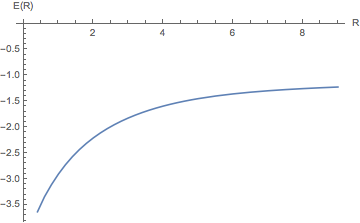
\includegraphics{Bates3DEofR.png}
\end{figure}

Total energy, calculated by adding the potential energy of the nuclei $ V(R) = 1/R $.

Electron energy as an eigenvalue of the equations \eqref{bandL} and \eqref{bandM}.
\begin{figure}
  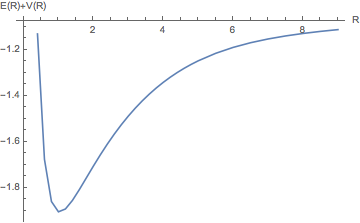
\includegraphics{Bates3DEofRPlusVofR.png}
\end{figure}

Table comparing the electron  energies obtain using our method vs method applied by Bates et al. We chose a subset of values to indicate the overall trend.

afterpage{
  \newgeometry{left=4em,right=3em,top=5em,bottom=5em}
  \captionsetup{type=figure}
  \captionof{table}{Electron Energy, \texorpdfstring{$ 1s\sigma_g $}{sigma g} state}
  \label{tab:UsVsBates}
    \begin{tabular}{ >{\bfseries}m{4em} m{4em}  m{4em}  m{4em} }
      \hline
      R & -E(R) (Bates) & -E(R) (out method)  \\ \hline \hline
      0.4 & 3.60157 & 3.632200 \\[-1em]
      0.6 & 3.34301 & 3.3429676 \\[-1em]
      0.8 & 3.10895 & 3.1089586 \\[-1em]
      1.0 & 2.90356 & 2.9035720 \\[-1em]
      1.2 & 2.72461 & 2.7246154 \\[-1em]
      1.4 & 2.56853 & 2.5685373 \\[-1em]
      1.6 & 2.43186 & 2.4318740 \\[-1em]
      1.8 & 2.31162 & 2.3116176 \\[-1em]
      2.0 & 2.20525 & 2.2052681 \\[-1em]
      2.2 & 2.11076 & 2.1107695 \\[-1em] 
      2.4 & 2.02642 & 2.0264405 \\[-1em]
      2.6 & 1.95090 & 1.9508966 \\[-1em]
      2.8 & 1.88299 & 1.8829977 \\[-1em]
      3.0 & 1.82178 & 1.8217919 \\[-1em]
      3.2 & 1.76647 & 1.7664850 \\[-1em]
      3.4 & 1.71639 & 1.7164029 \\[-1em]
      3.6 & 1.67097 & 1.6709739 \\[-1em]
      3.8 & 1.62971 & 1.6297050 \\[-1em]
      4.0 & 1.59216 & 1.5921695 \\[-1em]
      4.2 & 1.55799 & 1.5579948 \\[-1em]
      4.4 & 1.52685 & 1.5268516 \\[-1em]
      4.6 & 1.49844 & 1.4984480 \\[-1em]
      4.8 & 1.47252 & 1.472523 \\[-1em]
      5.0 & 1.44884 & 1.448840 \\[-1em]
    \hline
    \end{tabular}
}
